% LREC-COLING 2024 Example; 
% LREC Is now using templates similar to the ACL ones. 
\documentclass[10pt, a4paper]{article}

\usepackage[review]{lrec-coling2024} % this is the new style

% Custom packages
\usepackage{amsmath}


\title{Multimodal Language Models Show Evidence of Embodied Simulation}

\name{Cameron Jones, Sean Trott} 

\address{Department of Cognitive Science, UC San Diego \\
         9500 Gilman Drive, La Jolla, CA \\
         cameron@ucsd.edu, sttrott@ucsd.edu}


\abstract{
Multimodal large language models (MLLMs) are gaining popularity as partial solutions to the ``symbol grounding problem'' faced by language models trained on text alone. However, little is known about whether and how these multiple modalities are integrated. We draw inspiration from analogous work in human psycholinguistics on \textit{embodied simulation}, i.e., the hypothesis that language comprehension is \textit{grounded} in sensorimotor representations. We show that MLLMs are sensitive to \textit{implicit} visual features like object shape (e.g., ``The egg was in the skillet'' implies a frying egg rather than one in a shell). This suggests that MLLMs activate implicit information about object shape when it is implied by a verbal description of an event. We find mixed results for color and orientation, and rule out the possibility that this is due to models' insensitivity to those features in our dataset overall. We suggest that both human psycholinguistics and computational models of language could benefit from cross-pollination, e.g., with the potential to establish whether grounded representations play a \textit{functional} role in language processing.
 \\ \newline \Keywords{grounding, multimodal language models, embodiment} }

\begin{document}

\maketitleabstract

\section{Introduction}

Recent advances in Large Language Models (LLMs) have generated an explosion of interest in their underlying capabilities and limitations \cite{thirunavukarasu2023large}. One oft-cited limitation of contemporary LLMs is that they are trained on linguistic input alone \cite{bender2020climbing}, and thus, unlike humans, lack access to embodied experience---seen by some as a prerequisite for language understanding \cite{bisk2020experience, harnad1990symbol, mollo2023vector}.
Multimodal Large Language Models \cite[MLLMs][]{driess2023palm, girdhar2023imagebind, huang2023language}---which learn to associate linguistic representations with data from other modalities---may be a partial solution to this \textit{symbol grounding problem} \cite{harnad1990symbol}.
Yet despite impressive performance by MLLMs \cite{dosovitskiyImageWorth16x162021}, little is known about how distinct modalities (e.g., language and vision) are \textit{integrated} within a model's representational space, as they appear to be in humans.

We address this gap by turning to an analogous debate about the extent to which \textit{human} semantic representations are grounded in sensorimotor experience \cite{barsalou1999perceptual}. The \textit{embodied simulation hypothesis} \cite{bergen2015embodiment, glenberg2010embodiment} argues that language understanding involves the activation of grounded representations, i.e. that the same neural tissue recruited to perceive or participate in an event (e.g., kicking a soccer ball) is also engaged to understand language about that event (e.g., ``She kicked the ball''). Indeed, a wide body of experimental evidence suggests that some degree of sensorimotor activation occurs during language processing \cite{zwaanRevisitingMentalSimulation2012, winter2012language}. While there is ongoing debate about the functional relevance of embodied simulation \cite{glenberg2008use, mahon2008critical, montero2022no, ostarek2021towards}, the evidence points to some degree of cross-talk between linguistic and sensorimotor neural systems. 

Much of this evidence comes from the \textit{sentence-picture verification task} paradigm \cite{stanfield2001effect}. In this task, participants read a short sentence (e.g., ``He hammered the nail into the wall''), then see a picture of an object (e.g., a nail) and must decide whether the object was mentioned in the preceding sentence. Crucially, when the image of the object \textit{matches} the orientation (or shape, color, etc.) implied by the sentence (e.g., the nail is horizontal rather than vertical), participants are faster and more accurate in their decisions \cite{stanfield2001effect, pecher2009short, connell2007representing}. Because the object is the same (e.g., an egg), humans must be inferring visual features based on properties of the event itself (e.g., an egg cooking in a skillet).

In the current work, we applied these methodological insights to improve our understanding of MLLMs. We ask whether MLLM's internal representations of linguistic input (e.g., "He hammered the nail into the wall") are more similar to representations of images that \textit{match} visual features implied by that input than those that do not. To address this question, we adapted materials from three psycholinguistic studies that provide evidence for simulation of the implied orientation \cite{stanfield2001effect}, shape \cite{pecher2009short}, and color \cite{connell2007representing} of objects. Note that this approach differs from a standard classification task: rather than classifying images on the basis of which objects they contain (e.g., ``a cup of coffee'') or explicit features of those objects (e.g., ``a black cup of coffee''), we are asking whether the MLLM activates \textit{implicit} features that could be inferred from a more holistic event representation (e.g., ``Joanne never took milk in her coffee'' implies that the coffee is black). 

\begin{figure*}[ht]
    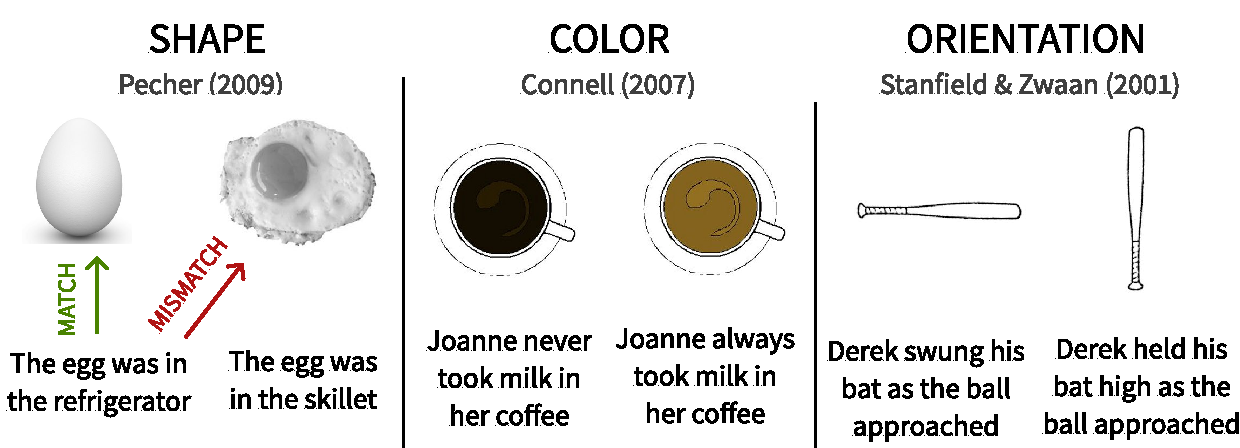
\includegraphics[width=\textwidth]{images/materials.pdf}
    \label{fig:materials}
    \caption{The dataset consisted of pairs of sentences and images, forming quadruplets. Each sentence in a pair implied that an object had a certain visual property (e.g. brown color). Each implied visual property was matched by one of the pair of images. The implied visual properties included \textsc{shape} \citep[\textbf{Left, }][]{pecher2009short}, \textsc{color} \citep[\textbf{Center}, ][]{connell2007representing}, and \textsc{orientation} \citep[\textbf{Right}, ][]{stanfield2001effect}.
    }
\end{figure*}

\section{Methods}

\subsection{Materials}

We used stimuli from three experiments that measured visual simulation in human participants. Items were organized as quadruplets, consisting of a pair of images and a pair of sentences.
Sentence pairs differed by implying that an object had a certain visual property (\textsc{shape}, \textsc{color}, or \textsc{orientation}).
Each of the images in a pair matched the implied visual feature in one of the sentences (and therefore mismatched the other, see Figure \ref{fig:materials}).

% Item description
60 quadruplets from \citet{pecher2009short} varied the implied \textsc{shape} of an object. A sentence such as ``There was an egg in the [refrigerator/skillet]'' implied that the egg was either in its shell or cracked open. A pair of black-and-white images of eggs matched one of these sentences by displaying the relevant visual feature.
% Connell
\citet{connell2007representing} collected 12 quadruplets that vary the implied \textsc{color} of an object. ``Joanne [never/always] took milk in her coffee'' implies black/brown coffee. The images differed only in color.
% Stanfield
Finally, \citet{stanfield2001effect} collected 24 quadruplets of sentences implying different \textsc{orientations} of an item, and line-drawings that were rotated to match the implied orientation. For instance ``Derek swung his bat as the ball approached'' suggests a horizontal bat, while ``Derek held his bat high as the ball approached'' suggests a vertical bat.


\subsection{Model Evaluation}

To probe MLLMs, we implemented a computational analogue of the sentence-picture verification task. Our primary question was whether a model's representation of a given linguistic input (e.g., "He hammered the nail into the wall") was more similar to its representation of an image that matched an implied visual feature (e.g. horizontal orientation) compared to an image that did not (e.g. a vertical nail).
% Technical explanation
For each sentence-image pair, we found the dot product between the MLLM embedding of the sentence and the image. This value quantifies the similarity between the linguistic and visual representations within the model. The dot product values were then passed through a softmax function, converting them into probabilities of the model associating eachimage with a given sentence:

\[ p_{ij} = \frac{\exp(S_i \cdot I_j)}{\sum_{k=1}^{2} \exp(S_i \cdot I_k)} \]

where \( S_i \) is the embedding for sentence \( i \), \( I_j \) is the embedding for image \( j \), and \( p_{ij} \) is the softmax probability that sentence \( i \) matches with image \( j \).
% Stats
To statistically evaluate the model's performance, we conducted a t-test to compare the probabilities of matching (e.g., \( p_{11} \) and \( p_{22} \)) against mismatching (e.g., \( p_{12} \) and \( p_{21} \)) sentence-image pairs. A significant result, where the matching probabilities are greater than mismatching ones, would indicate that the MLLM's representations are sensitive to the visual properties implied by the linguistic input.

\subsection{Vision-Language Models}

We evaluate four different CLIP-based Vision Transformers with different numbers of parameters and training regimes in order to test the generalizability and robustness of implied visual feature effects.

% ViT explanation
The Vision Transformer (ViT) architecture adapts the Transformer to handle visual data \cite{dosovitskiyImageWorth16x162021}. The ViT divides an image into fixed-size non-overlapping patches that are then linearly embedded into input vectors.
A classification head is attached to the output to produce the final prediction. Despite their simplicity and lack of inductive biases (e.g., convolutional layers), ViTs have achieved competitive performance on various visual tasks, especially when pre-trained on large datasets \cite{dosovitskiyImageWorth16x162021, schuhmannLaion5bOpenLargescale2022}.

CLIP (Contrastive Language–Image Pre-training) employs contrastive learning to associate images with text descriptions \citep{radfordLearningTransferableVisual2021a}. The model jointly trains a ViT image encoder and a text encoder to predict the correct pairings of (image, text) pairs. This allows CLIP to learn a shared semantic space between images and text. We evaluate four pre-trained CLIP models:

\textbf{ViT-B/32}: The base model from \citep{radfordLearningTransferableVisual2021a}. ViT-B/32 uses a patch size of 32px and has 120M parameters. It was trained on 400 million 224x224 pixel image-text pairs over 32 epochs.

\textbf{ViT-L/14}: The best-performing model from \citep[described in the paper as ViT-L/14@336px]{radfordLearningTransferableVisual2021a}. ViT-L/14 uses a patch size of 14px and has 430M parameters. It was pre-trained in the same manner as ViT-B/32 and then fine-tuned at 336px for one additional epoch.

\textbf{ViT-H/14}: A larger model based on the CLIP architecture \citep{ilharco_gabriel_2021_5143773}. ViT-H/14 has 1B parameters and was trained on the LAION 2B dataset for 16 epochs \cite{schuhmannLaion5bOpenLargescale2022}.

\textbf{ImageBind}: an MLLM that learns a joint embedding across six modalities, including images, text, audio, depth, thermal, and IMU data \cite{girdhar2023imagebind}. Internally, a Transformer architecture is used for all modalities. The image and text encoders are based on the ViT-H/14 model.

% \begin{table}[h]
%     \centering
%     \begin{tabular}{|m{0.25\columnwidth}|m{0.3\columnwidth}|m{0.2\columnwidth}|}
%         \hline
%         Sentence & Image Match & Feature \\
%         \hline
%         \\There was apple pie on the table.& 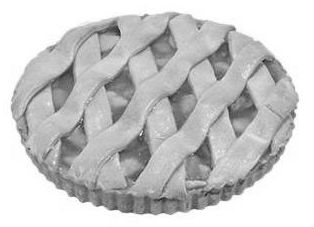
\includegraphics[width=0.2\columnwidth]{images/applepie.jpg} &
%         Shape \\
%         \hline
%         \\There was apple pie on the plate.& 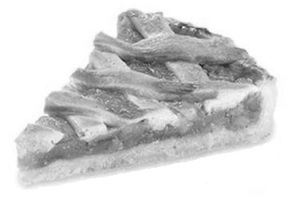
\includegraphics[width=0.2\columnwidth]{images/applepieslice.jpg} &
%         Shape \\
%         \hline
%         \\Derek held his bat high as the ball approached.& 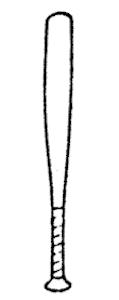
\includegraphics[height = .2\columnwidth]{images/batV.jpg} &
%         Orientation\\
%         \hline
%         \\Derek swung his bat as the ball approached.& 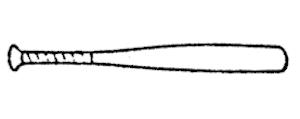
\includegraphics[width = .2\columnwidth]{images/batH.jpg} &
%         Orientation \\
%         \hline
%     \end{tabular}
%     \caption{Sentences and matching images taken from psycholinguistic studies \cite{pecher2009short, stanfield2001effect, connell2007representing}.}
%     \label{tab:sample_table}
% \end{table}

\section{Results}

We tested whether MLLMs were sensitive to the implied visual features in the sentence using a t-test.
The test compared the probability assigned to images that matched the implied visual features versus those that did not.
All of the models, except for the smallest (ViT-B/32), showed a significant effect of \textsc{shape}.
ImageBind showed the largest effect: $t(238) = 4.65, p < 0.001$.
ViT-B/32 showed an effect in the expected direction but it did not reach significance: $t(238) = 1.81, p = 0.072$.

The results for \textsc{Color} were more varied. Neither the ViT-B/32 and ViT-L/14 models showed a significant effect of match between the color implied by a sentence and the color of an image.
Both ViT-H/14 ($t(46) = 2.16, p < 0.05$) and ImageBind ($t(46) = 2.85, p < 0.01$ demonstrated sensitivity to implied color properties although these effects were less robust than for shape.

None of the models showed significant sensitivity to implied \textsc{orientation} from linguistic cues. The largest numerical effect was shown by ImageBind: $t(94) = 1.09, p = 0.278$ (see Table \ref{tab:results}).

\begin{figure*}[ht]
    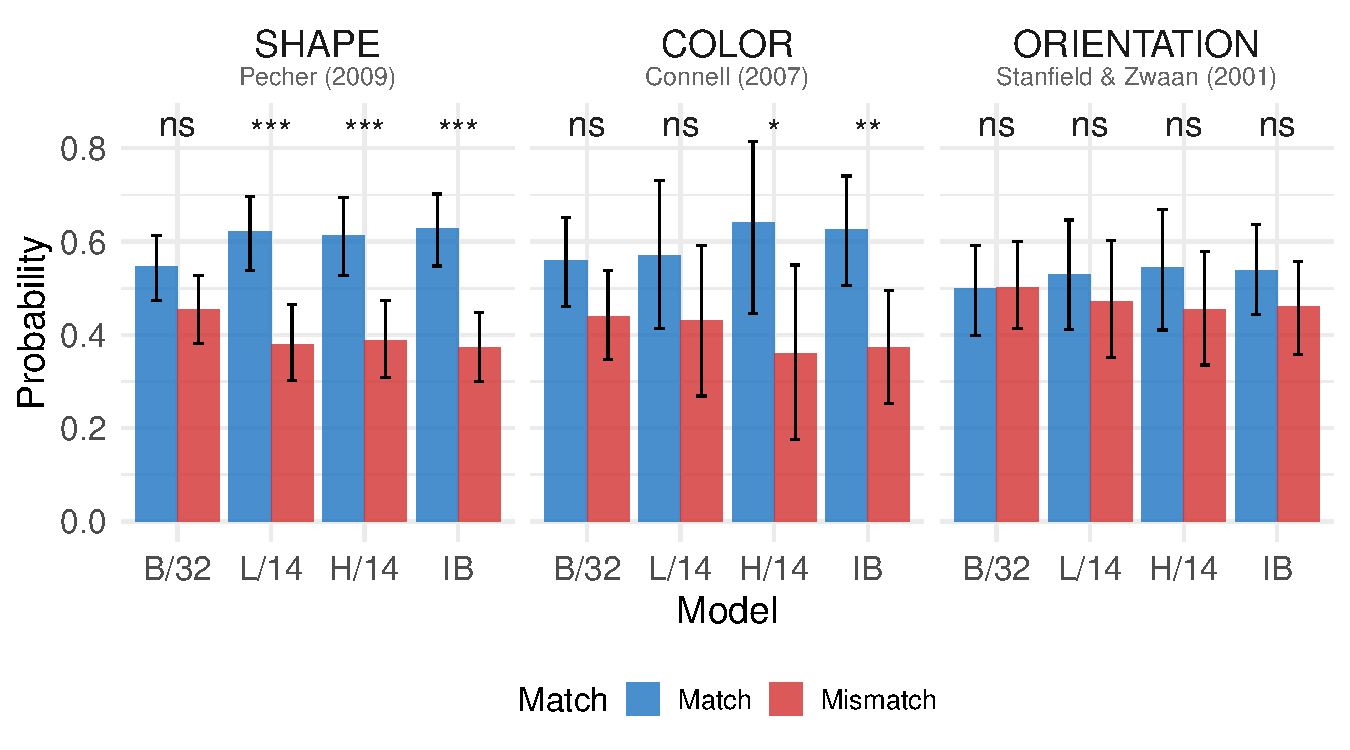
\includegraphics[width=\textwidth]{images/results.pdf}
    \label{fig:results}
    \caption{Comparison of mean probability values assigned to images that either matched (blue bars) or did not match (red bars) implied visual features of a sentence. Four Vision Transformer Models (ViT-\textbf{B/32}, ViT-\textbf{L/14}, ViT-\textbf{H/14}, and \textbf{I}mage\textbf{B}ind)), were evaluated across three datasets (\textsc{Shape}, \textsc{Orientation}, and \textsc{Color}). Error bars denote 95\% bootstrapped confidence intervals.}

\end{figure*}

\begin{table}[ht]
\label{tab:results}
\centering
\begin{tabular}{lrrr}
  \hline
Model & Shape & Color & Orientation \\ 
  \hline
ViT-B/32 & 0.072 & 0.112 & 0.965 \\ 
  ViT-L/14 & \textbf{<0.001} & 0.240 & 0.510 \\ 
  ViT-H/14 & \textbf{<0.001} & \textbf{0.036} & 0.323 \\ 
  ImageBind & \textbf{<0.001} & \textbf{0.006} & 0.278 \\ 
   \hline
\end{tabular}
\caption{p-values from t-tests measuring the effect of matching implied visual features between labels and images. All models except ViT-B/32 show a significant effect for \textsc{Shape}. ViT-H/14 and ImageBind both show significant effects for \textsc{Color}. None of the models show an effect of \textsc{Orientation}.} 
\end{table}


\subsection{Follow-up Analysis of Explicit Features}\label{sec:followup}

One potential explanation for the null results reported above is that MLLMs are insensitive to the manipulated visual features like orientation, or that these features are difficult to identify in the image stimuli used.
To test this possibility, we ran a follow-up ``manipulation check'' to determine whether the MLLMs were sensitive to orientation and color when they were explicitly mentioned in the text. The analysis was virtually identical to the primary analysis above, except that we used a sentence template that \textit{explicitly} described specific visual features of the object in question, e.g., ``It was a [COLOR] [OBJECT]''. We then asked whether the MLLMs could successfully match sentences with explicit visual features (e.g., ``It was a red traffic light'' vs. ``It was a green traffic light'').

All models tested showed an effect of both \textsc{color} ($p < .01$) and \textsc{orientation} ($p < .01$). That is, models assigned higher probability to images with visual features that matched those \textit{explicitly mentioned} in the sentence. This indicates that the MLLMs are sensitive to \textsc{color} and \textsc{orientation}, and that stimulus quality is sufficient to identify these features.

\section{Discussion}

Our central question was whether MLLMs showed effects that have been taken as evidence of embodied simulation in humans \cite{stanfield2001effect}. We asked whether MLLMs were sensitive to specific visual features (shape, color, and orientation) that were \textit{implied} but not explicitly mentioned by a verbal description of an event. We found robust evidence of simulation for implied \textsc{shape}, mixed evidence for simulation of implied \textsc{color}, and no evidence of simulation for implied \textsc{orientation}.
 
Importantly, none of these visual features were explicitly mentioned in the sentences. Thus, if an MLLM exhibits sensitivity to implied \textsc{shape}, it suggests that the model is activating \textit{event-specific} representations of the objects mentioned in a sentence. In humans, an analogous effect is taken as evidence of embodied simulation \cite{stanfield2001effect, bergen2015embodiment}. The findings here suggest that such an effect can be produced via exposure to large-scale statistical associations between patterns in images and patterns in text.

It is unclear why MLLMs did not appear to simulate orientation (or color, in some cases). Critically, when either feature was \textit{explicit} in the text, a match effect was obtained (see Section \ref{sec:followup}); this suggests the null effects were not due to overall insensitivity to those visual features. Instead, MLLMs appear to activate some implicit visual features more readily than others.
This variation could be driven by noise in the relationship between images and descriptions. Orientation can be influenced by rotation or viewpoints and color similarly varies with lighting.
Implicit indications of these features in text labels may therefore be less reliable than indications of more invariant features such as shape.
Future work could ask whether color and orientation are \textit{less integrated} with linguistic representations in MLLMs, or simply harder to infer from text descriptions.

Future studies could also explore whether MLLMs simulate modalities beyond vision. There is evidence that humans activate other sensorimotor modalities, such as auditory volume \cite{winter2012language} and motor action \cite{fischer2008embodied}, though evidence for other modalities like olfaction is limited \cite{speed2018exception}. 

Finally, there is considerable debate within psycholinguistics over whether embodied simulation plays a \textit{functional} role in language comprehension, or whether it is epiphenomenal \cite{ostarek2021towards, mahon2008critical, glenberg2008use}. Future work could contribute to this debate by using MLLMs as ``subjects'': specifically, researchers could ``lesion'' representations of features like \textsc{shape} and ask whether this causally affects processing of sentences implying object shape. This would join the broader ``neuroconnectionist'' research program that aims to unify research on human cognition and on models inspired by cognition \cite{doerig2023neuroconnectionist}.

\section{Conclusion}

We found that MLLMs are sensitive to whether visual features that are \textit{implied} by a sentence are matched in an image, a phenomenon taken as evidence of embodied simulation in humans.





% \section{Acknowledgements}

% We thank Louise Connell for providing her stimuli.



\section{Ethical Considerations and Limitations}

The study is limited in that it only evaluates Vision Transformers. Other VLM architectures may produce different associations between text and images.
The number of items for some of the datasets was small. Some models may have shown significant match effects with a larger number of items.
One potential limitation of the study is that the tasks given to human and LLM participants are not quite analogous.
In the picture-verification task, the participant is aware that the implied visual features are irrelevant: their task is to identify whether the object was present in the sentence.
The models cannot be so instructed: the measure of association between the sentence and image representations will be based on all features that were useful to the model during CLIP pre-training.
Nevertheless, the results show that models are sensitive to these implied features even when they are not explicitly mentioned.


% \nocite{*}
\section{Bibliographical References}\label{sec:reference}

\bibliographystyle{lrec-coling2024-natbib}
% \bibliography{lrec-coling2024-example}
\bibliography{embodiment}

% \section{Language Resource References}
\label{lr:ref}
\bibliographystylelanguageresource{lrec-coling2024-natbib}
\bibliographylanguageresource{languageresource}


\end{document}

%%% Local Variables:
%%% mode: latex
%%% TeX-master: t
%%% End:
